%!TEX root = dissertation.tex

\chapter*{About this project}
\paragraph{Abstract}

Dúchas Na Gaillimhe ( Galway Civic Trust ) along with Tourism Ireland carry out walking tours of Galway city to inform visitors of Galway's long and rich history. One of the walks they offer tourists during the summer months is a medieval walking tour of Galway city. This walk visits seven locations starting at the Hall of the Red Earl in Galway’s Latin Quarter. However, this limits visitors to attending guide-lead tours at specific times as well as only being available frequently during the summer tourist season.

This project aims to deliver a solution which helps tourists visiting Galway city to take the medieval walking tour of Galway at any time, without the need of a guide and will be available at any time of the year. If the tourist wishes to seek further information they can drop into Galway Civic Trust's office which is located at the Hall of the Red Earl.

The proposed solution will comprise a mobile phone application which will allow users to be guided around Galway city. It will show the user their current location and the destination they wish to reach. On arrival at the destination, the app provides the user with information and images about the location. A user can get additional information if they so wish. There will also be a web application used by Galway Civic Trust personnel to update the information on the application periodically and make it automatically available to all new and existing app users accessing the database.

\paragraph{Authors}
Sarah Carroll, Abigail Culkin
B.Sc.(Hons) in Software Development

\chapter{Introduction}

At the beginning of Year 4 in Software Development at GMIT, the authors were given the opportunity to work on the Medieval walking tour project for an external small/medium Enterprise organised through GMIT. The idea of the project is based on the problem that medieval walking tours of Galway city are not always available for tourists at convenient times and infrequently outside the main summer season. 

The purpose of this Final Year Project is to build an application using new technologies that the developers have never used before. Therefore, it allows for research to be done, learn up and coming technologies and discover new ways of developing software. The front-end technology being used to create the mobile application is Flutter. It will be connected to a backend server running on Google cloud platform and within this a MongoDB Flask Database which uses docker. Working with Galway Civic trust allowed for an application to be made that is missing from the market place for Galway tourism. This application will be useful and easy to use for customers and the company will benefit from this.  This way, the authors will be able to show they have worked with an outside source and have a fully functioning app that will satisfy what was asked of them.

The technologies used will be explained and why we used them throughout. The research and development will all be detailed and allow others to understand why specific software was chosen. This project is done using technologies that have not been used together too often. This means any problems faced or certain aspects found to be new will be documented along with the development.
\section{Context}

\subsection{Context of the Project}
The context of this project revolves around the use case of being a tourist in Galway city, wishing to find out more information about the city's history. Opening the app on the user’s phone, they can view their location in relation to the locations on the guided tour. This application prevents the user getting lost and gives them accurate information about each location. The information on the application was provided by Galway Civic Trust and is the same information a tourist gets on the guided walking tours. Reading the data and retrieving images from the database needs to be very fast, as any delayed hang in performance could lead to a bad user experience.

The project will be developed as a Cross-Platform application which provides users with images, information and a map of Galway city and the seven medieval stops along the tour. Users of the application can get their location in relation to the exact location of the points of the tour at any given time. When the user decides they wish to learn more information about a specific location, they can retrieve images and text about the location on the application. Along with the mobile application a web application will be developed for use by Galway Civic Trust personnel to update, delete or add information to the tours database.

\section{Objectives} 

The project will require a number of objectives to be accomplished in order to provide a solution that works and is suitable for the use of Galway Civic Trust. 

\begin{itemize}
\item A Mongo database will be used to store the text which appears in the application. This database will need to be setup and hosted in such a way that it can be accessed from clients through the Flutter application. The database will be hosted on Amazon Web Services Cloud.

\item A client application will be the main product / asset for the project. This application will be able to locate the user via the GPS on their mobile device. The app will then show the user the locations of each point on the tour. This will provide the user an idea of how far they are from the chosen point and will allow them to see when they have reached their destination. Each location is specified on the application as a list on the home page. Then chosen images and information will appear for each location. When clients wish to get more information about a certain location they can do so by clicking "More Information" button.

\item An additional requirement is to develop a web application for the use of the company to allow them to modify the information shown to the user. The web application is a simple website that can access the database to create, update and delete information from the database.

\item Using the Google Maps application programming interface (API) within the mobile application to show the user their location along with the specific points of the tour. Each location is indicated by a marker in the map. When the user clicks on a specific marker the name of the location appears as a label.

\item Pull information from the Mongo DB using flask.


\end{itemize}
\section{Overview}

Each Chapter of this paper will contain different details regarding the project. 

The Background chapter will discuss the rationale behind the project, the collaboration with Galway Civic Trust, technologies selection and explain each technology used in detail.

The Methodologies chapter will describe the way in which software development and research methodology was addressed. The aids used to help working in a team will also be discussed. The way in which each technology was used, system integration and system architecture will be outlined also.

The results Chapter will discuss the results of the application including screenshots. It will also discuss limitations and difficulties encountered throughout the project life cycle. This chapter will also go into detail on different types of testing suitable for this project.

The conclusion briefly summarises the project, reflecting on the objectives of the project.

\chapter{Background}
\section{Rationale}
This Project is created in order to provide an application to be used for Galway Tourism as well as to fulfill the criteria laid out for a final year project in Computing and Software Development. It will be used by Galway Civic Trust and will be published to the Google Play android store and the IOS app store. It will with meeting the standards required for a Level 8 final year project. The client application is developed using Google’s Flutter UI framework - this was a new framework to the developers. This is used in conjunction with MongoDB flask. The admin application is developed in Angularjs and connects to the MongoDB flask backend. This is also new technology to the developers and therefore the project brings great learning experience along with a lot of background research.

\section{Collaboration}
This project is created in collaboration with Galway Civic Trust. Galway Civic Trust is an organisation located at the Hall of the Red Earl, Custom House, Druid Lane, Galway. The idea came about through the mentor for this project, Brian Mcginley. The organisation has been looking to create an application for their walking tours around Galway city. This application will enable the easy accessibility of information for tourists. All images and information included in this application was provided by Galway Civic Trust.

\section{Technology Selection}
During the initial planning of this project, the frameworks considered included Ionic, Flutter, React native, native applications and Xamarin. The winner was the Flutter framework. This is a new framework introduced by Google. It is built using the Dart programming language. Flutter has multiple benefits including its simplicity to be used for cross platform applications.


\subsection{Flutter vs native languages}
Native applications for Android are built in Java or Kotlin, and native applications for ISO are generally build in Swift. When developing in Flutter there is a single code base. This means the application is written once and it works for both IOS and Android. Third Party libraries are widely available for native language applications. This is due to the popularity of their language and therefore there are very few problems that can not be solved by referencing Stack overflow, etc. Because Flutter is relatively new the third party libraries are limited, new libraries are coming available each day due to the trust companies have in Google’s ability to deliver. Native languages and Flutter both give a native application appearance. "Well-written native code should always be more performant than compiled native code." \cite{FlutterVS_2018}.The executable file size for a Flutter application is much larger then the equivalent application for native languages.On flutter platform specific functions such as gps and camera functionality needs to be defining specifically for each ios and android.The implementations of these features is the same as implementing in platform native languages.\cite{flutter_application}

\subsection{Flutter vs Xamerin}
Flutter is maintained on a single code base for all platforms. This enables simplicity for testing and reduces development time. For this reason it was chosen over the Xamerin framework. Xamerin is a C Sharp based platform. Flutter offers APIs and SDKs for 2D rendering, simulation, gestures, and painting as well as allowing the use of existing Swift, Objective C, and Java code. It comes with Machine Design Widgets, also a Google product. \cite{flutterVsXamarin}Xamerin is hardware consistent meaning it had a large variety of apis available to enable a friendly user experience. Flutter is also hardware consistent. Flutter applications are backward compatible with older versions of ISO and Android.\cite{flutterVsReactVsXamarin}

\subsection{Flutter vs React Native}
React Native is similar to Flutter and compiles to native application by default. A basic React Native application is given a basic set of components. The developer must style most of them separately for each platform. This creates more work for the developer and increases time of development and cost of development for a company. React Native is developed by Facebook, while Flutter is created by Google. Each company is well developed and looked upon favourably by smaller businesses. React Native applications are developed using Javascript and React libraries to build user interfaces. React previously existed to create web applications. Flutter is developed using the Dart programming language and is soley used for mobile application development. React is a very popular language with 65K starts on github in comparison to 30K for Flutter. However Flutter is becoming more and more popular. \cite{FlutterVS_2018} \cite{ReactVsFlutterVsIonic}

\subsection{Flutter vs Ionic}
Flutter and Ionic are very similar in what they offer with regards to pre-built components in Flutter and a comprehensive suite of built in widgets in Ionic \cite{ReactVsFlutterVsIonic}. With Ionic, you create a real native app but you do this by creating a web app (with Hyper Text Markup Language, JavaScript and Cascading Style Sheets) which will be wrapped by a real native app that hosts a web view while Flutter you write Dart code which can be compiled to native code that runs on the target device. The main reasoning for using Flutter over Ionic is that it is new. It is powered by Google and therefore is well documented and although it’s still new there are loads of interactive talks online about the upcoming and new features of Flutter. Ionic has numerous third party built in tools. It has thousands of threads on Stackoverflow and packages on NPM (node.js package manager) to help developers along the way.\cite{FlutterVS_2018}

\section{Technology}
\subsection{Server}
\subsubsection{MongoDB}
MongoDB is one of many nonrelational databases. It is a NoSQL database that is used across many areas in the technology and business sector. MongoDB is a free open source database management system. As it has evolved over the years it is now one of the most popular document orientated databases. It is run on a mongo server and can be created and controlled from your command prompt. Data in MongoDB is stored in JSON like documents. A format called BSON which is JSON in binary style is used for document storage in the database.\cite{MongoDB} This allows for an easy to read format of the data. Dissimilar to relational databases for example MySQL which uses rows and tables as a database structure MongoDB is formed of collections and documents. Each database in mongo can have multiple collections. "A collection is a group of documents".\cite{MongoDBColections} These documents can have many fields. The Documents in the database are a set of key value pairs. An id will be assigned to the documents making your database easy to edit. As MongoDB is a NoSQL nonrelation database it differs in many ways from a relational database management system. A relational database is row and column based as opposed to document and field based.\cite{MongoDBColections} MongoDB is considerably easier to set up and is not vulnerable to SQL injection. A RDMS can more challenging to understand and lets down the database in terms of its hierarchical storage not being as good and how it is open to SQL injection. One of the more popular relational databases is MySQL. Compared to MongoDB it is quite inflexible in terms of the database schema. \cite{MongoDB} MongoDB is known for its ability to "handle large amounts of unstructured data" which MySQL lacks in its technical features. \cite{MongoVsMysql} Improving databases in terms of storage and their schemas can help to build more efficient and easier to understand technologies. MongoDB runs better than many other database systems used today. It is a high-quality technology which has features that are desirable in having a secure database. Known for its scalability, memory processing and concurrency MongoDB makes for a desired database. All these features make it easy to develop a fast, reliable database which makes it work alongside evolving applications and is sought after by businesses. It is flexible and can be adapted to work with many platforms and can be integrated into software much easier than other database management systems. The most common frameworks that are used in conjunction with MongoDB are NodeJS and a newer one Mongo Flask. It is also supported by cloud services such as Amazon Web services and google cloud platform.

\subsubsection{Flask}
Flask is a web framework which is programmed in python. Flask can support many extensions that can be used for adding specific features to the framework. A flask web application is written using simple python to start with. It can be "used for developing we applications, wikis or commercial websites".\cite{FlaskInfo} The webpage uses a static file to display the information which is designed using html and CSS. It contains a built-in development server and debugger. It also supports integrated unit testing which means flask is adding features to adapt to new technologies. There are no restrictions on the flask application architecture or on the data abstractions layers. There is a large amount of documentation on how to run flask with python how to set it up. Within flask you can use PyMongo. "PyMongo contains tools for integrating with MongoDB and Python".\cite{PyMongo} This can be imported in the flask web framework in your python file. The BSON format is also in python and PyMongo. This will allow us to read the database as readable text as MongoDB uses JSON like documentation.\cite{PyMongo} You can adapt your python to talk to your database in a simple way. "Flask uses a database URL" to connect all information in the database to produce get access to data from your database.\cite{FlaskPy} Flask can be run on a cloud service which allows you to run your web page through open ports and run it remotely from your own IP address. In the flask and Python, it is HTTP methods that are used for communicating with the database which will allow you can read it and edit any information. \cite{FlaskPy} Flask is one of Pythons most popular web frameworks. Flask would not be as known or as popular as NodeJS and Express when it comes to connecting to databases or integrating database URLs. Flask is known for being easy to use and this is good for beginners and quick web page building. \cite{Flask} Node and Express is much more advanced including their libraries and more complex tasks that can be added into a NodeJS platform therefore it is more difficult.\cite{FlaskVNode}
\subsubsection{Docker}
Docker is an open source tool which uses containers to make it easier to develop applications.\cite{DockerCont} The containers allow you to create an application uses a package containing any part needed to create and deploy your application. These packages can supply such things as libraries and dependencies. This means that separate downloads are not needed, and any Linux machine can run this app as Docker will supply any libraries needed. Docker is run on the Linux kernel. It was created to make developing focus on the writing and not the systems needed to run or set up the application. It provides security to your software. The main aim of a container is to ensure your software runs quickly and safely from one system to another. It is convenient as it can "run on Linux or Windows based machines".\cite{Container} More than one docker container can be run on the same machine at once. They do not take up as much space as other systems like virtual machines for example. Google cloud platform and other virtual machines have made it easier to set up docker containers for your app that can be deployed remotely.\cite{DockerVsVm} Containers have great features that make them so popular for example you can run commands from the root, have processing space.\cite{DockerVsVm} One feature containers are desired for is they share their system kernel with other containers which similar technology like virtual machines cannot do. Overall Docker gives you more time spent on the software of your application and uses less hardware. Your processing power is much better with Docker which means a better performance rate for operating systems. The technology is easy download all done from your shell script. The Docker container is known for being the best running container available now for application development. When your database is running on a server it will be in one container and your application framework will be in another. Docker allows you link them easily creating great scalability. 

\subsection{client}
\subsubsection{Web Application}

\subsubsection{Mobile Application}
In order to develop the mobile application, Flutter was used. Flutter is an open source mobile application framework created by Google, developed in the Dart programming language. It is cross platform and therefore can create native applications for both Android and IOS from a single code base. Flutters first stable release was version 1.0 which was released on 4th December 2018. This was after the beginning of the development stage of this project. Therefore, until that date the beta testing version was being used. The preview release was made publicly available in September 2018. Although Flutter is an relatively new framework it is backed by a large range of documentation called Fluttterdocs. Flutter has a lot of positives and some negatives also came to light throughout this project.

\subsubsection{Widgets}
Flutter is made up of basic building blocks called widgets. Widgets help to create a immutable user interface. Flutter is made up of stateful widgets, stateless widgets, inherited widgets and keys. Flutter is made up of thousands of widgets each having their own purpose. These widgets are stacked on top of /within one another. An example of a simple widget is a padding widget on a text widget. The process of interlinking widgets together is called "composing". The widget that can hold other widgets within it is known as a container widget.\cite{widgets}

\subsubsection{Stateless widget}
Stateless widgets are only drawn once, this happens when the widget is loaded. These widgets are useful when the widget does not need a mutable state and is not used other then at the beginning when the information is passed to the object. Examples of stateless widgets include "text widget", "raised button widget" and "icon widget". The information passed into a text widget can be provided via a constructor or hard coded information. This therefore can not be changed by the user and is constant. This makes it a stateless widget. \cite{birch_2019}. From the code example below, the checkbox when clicked does not change without the page being reloaded.\cite{stateful_widgets_2018}.

\begin{figure}[ht!]
    \centering
 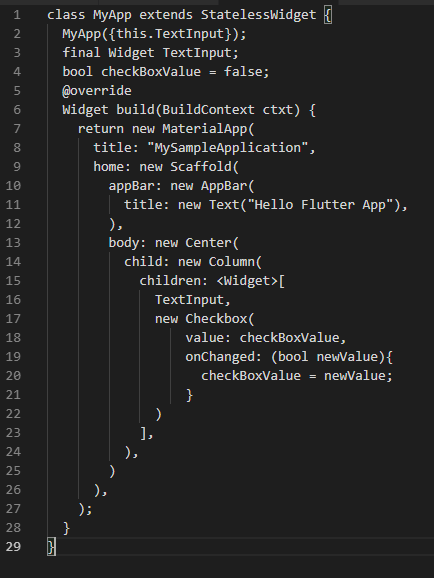
\includegraphics[width=75mm, height=75mm,scale=0.5]{img/stateless.PNG}
\caption{Code sample for stateless widget}
\label{fig:stateless}
\end{figure}

\subsubsection{Stateful widget}
Stateful widgets are dynamic and have a mutable state. Stateful widgets are widgets which can be read synchronously, when it is created and may change over the lifetime of the widget.\cite{stateful_widgets_2018}. The state can be reloaded by called the setState() method. In order to create a Stateful widget two classes must be made. One of which is created by extending statefulwidget (called myApp) and and another is created by extending the generic state<myApp>(this class is called myAppState). The typical hierarchy structure of a Stateful widget is matericalApp/home/scaffold/body/center/row/column/checkbox.\cite{widgets} \cite{stateful} Stateful widgets idea was originally taken from React Native e.g. the state can not  be changed outside of the state. A real example as to when a stateful widget is used is when having a button on a page such as a like button in order to keep track of how many times this button is pressed by the user the button must be located within a Stateful widget class. \cite{choudhary_2019}


\begin{figure}[ht!]
    \centering
 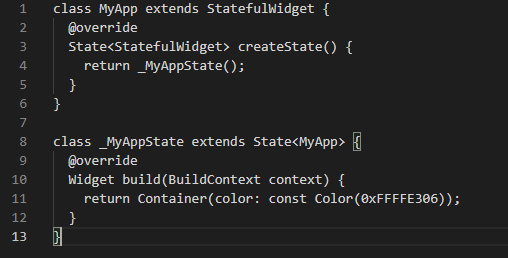
\includegraphics[width=75mm, height=75mm,scale=0.5]{img/stateful.PNG}
\caption{Code sample for stateful widget}
\label{fig:stateful}
\end{figure}

\subsubsection{inherited widgets}
An inherited widget is needed when the widget hierarchy gets very large and  information needs to be passed or accessed from a lower branch of the structure. A inheritied widget is a widget that can get called directly from any wiget in the tree structure below it. Inherited widgets are ideally kept small for good coding practise.\cite{fidanboylu_2019}.Theme is a type of inherited widget. It can be used in the context theme.of(context).primaryColor. This gets the global theme of a material app. An inherited widget is not able to be changed over time. Similar to stateless widgets they can only be replaced by rebuilding the entire widget.\cite{inherited_widgets}. Inherited widgets have a special unique method called "of". This method can access properties from anywhere on the widget tree.\cite{inheritedwidget_2018}

\subsubsection{Keys}
A key in Flutter is an identifier for widgets and elements. These are rarely used but when used they are ideal for preserving a scroll location and keeping the state when modifying a collection or database.\cite{key_widgets}A to do list application is an example of a time that a key would be useful. Adding, updating, removing and creating items in a collection. Keys are only necessary if the entire sub-tree is stateless. Keys enable the item to be stateful and enables the sub-tree to keep track of the items state when the widget is reloaded. \cite{keys}

\subsubsection{Advantages of Flutter}

\subsubsection{Fast Code Development}
Flutter offers Fast Code Development - this is due to the fact that it is a single code base for both Android and IOS development. This is known as a cross platform framework. All applications developed in Flutter are 2D. Flutter also offers a "hot reload" this enables users to work with developers and easily see changes been made. This hot reload is done in the command prompt which the application is running. Hot reload works by injecting updated source code into the running application on the dart virtual machine.\cite{faq_2019}
\subsubsection{Open Source}
Flutter is an open source framework. It is created by Google and has a large community which means the documentation is extensive and the Dart language is becoming more popular. Flutter has numerous built-in API's to support use of camera, geolocation, network storage and more.\cite{pros_cons}
\subsubsection{Less Code}
There is less actual code to write when using Flutter. Flutter is programmed in Dart. This is an object oriented programming language. Dart has similarities to React-Native because its programming style is reactive and declarative.\cite{pros_cons} Reactive coding ensures only having to declare something once in the code base. This ensures that there is less code to write along with the fact that is becomes more readable and reusable.\cite{depth_flutter_2019}
\subsubsection{Model View Presenter (MVP)}
Flutter is ideal for MVP (Model, View, Presenter) programming pattern. The MVP is replacing the MVC, the controller is exchanged for the presenter. This is a good idea because it enables the developer to create an application to show the customers very fast on both IOS and Android on one code base saving time.\cite{pros_cons}.

\subsubsection{Disadvantages of Flutter}

\subsubsection{Mobile Development alone}
Flutter caters to mobile development alone.(Andriod and IOS). Flutter is currently unable to create web applications. This is a limitation and may be a reason a company would opt against using Flutter.

\subsubsection{Lack Third party libraries}
Flutter is limited due the amount of third party libraries available to it. This is due to the fact that it is relatively new on the market and is based on Dart.\cite{pros_cons} React-Native has fully extensive third party libraries. It is based on JavaScript so therefore there were already libraries it could use when created. Dart was created by Google also. Therefore it has not developed many external libraries. However these libraries are growing every day. Flutter takes care of User Interface packages needs with widgets. Long term development can be limited.\cite{good_bad}

\subsubsection{Large File Size}
Flutter’s application size is much larger then native applications. The original “hello world” application in Flutter was 6.7mb. After many complaints from developers, the Flutter team managed to reduce the size to 4.7mb. At this, the simple hello world application is still very large in comparison to Java at 539kb and Kotlin at 550kb.\cite{faq_2019} \cite{good_bad}



\chapter{Methodology}
\section{Project Management}

Project Management is a key element of any task to ensure that the project is laid out correctly and each component part is complete at a given date etc. Because this project was completed by a team it was important both members completed each task. In order to track the project a Gantt chart was used. This broke down each step of the project and the expected time limits for each section.

\subsection{Agile}

The project used Agile project management methodologies. An iterative approach was taken. This meant that each week certain tasks are completed. The project team meet 3 times a week to discuss what has been completed since the last meeting, what has to be completed before the next and discuss any difficulties experienced thought out the duration. The meetings are short and concise. Once a week the team met their mentor and explained what was completed since the last meeting and is to be done before the next. These weekly meetings were the iterative approach. Each week the process would be repeated to meet, plan, design, develop, test and evaluate.

\begin{figure}[ht!]
    \centering
 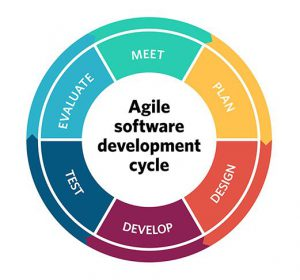
\includegraphics[width=75mm, height=75mm,scale=0.5]{img/agile.jpg}
\caption{Agile Life Cycle}
\label{fig:agile}
\end{figure}

\subsubsection{Agile Roadmap/gantt chart}
An agile Roadmap/gantt chart in agile development to help state the goals of the project from the outset.It helps break down the tasks which are then further broken down for sprints. This is usually a high level view of the project.\cite{testPlan} It is used often in industry and it helps to understand a project as a whole and learn what other teams are contributing to the overall project. The roadmap also shows how the project is likely to show how the project is likely to grow in the future. This is shown to the stakeholders and gives a better indication for funding etc.\cite{roadmap_2016}

\subsubsection{Planning and development phase}
During the meeting and planning phase. The milestones for the project were identified and broken down into simpler, more manageable tasks. The tasks are then grouped into sprints or iterations lasting one week each(in inductry normally 1/3 weeks). These are the tasks which must be be complete before each meeting. Each sprint started after the weekly meeting with the supervisor and the aim is for the work to be complete beofore the meeting the following week.\cite{Agile}.The plans for the project and the sprints are taken from the user stories.Development iterations convert the iteration plan into working code.\cite{agile_process}

\subsubsection{Design phase}
Throughout the agile development life cycle design is a step in every iteration/sprint. The design is graduallt built on.The design is never definded at the beginning of the project. The gradual evolution of the design enables taking advantage of new technologies that come insteam aswell as meeting any new requirements brought forward by clients. The user experience is key when designing a project/application.Every design must be user friendly.The type of end user of the item must be considered when designing.

\subsubsection{Testing}
Testing was carried out after multiple iterations. When tasks were complete that were stated in the test plan the tests were carried out.The user tests were carried out when meeting with the client.The client used the applications and commented any changed that were to be made.


\subsubsection{Evaluation Phase}
After each sprint before the meeting phase a review was carried out on the tasks completed in the last sprint. If there were changes to make these were completed in the next sprint. In the evaluation section of the agile development cycle the code by both developers was mergers into the master branch of the GitHub repository.The evaluation process is also used to look back, see how much of the previous iteration that was not complete and change the workload applied for a single iteration.\cite{agile_process}


\begin{figure}[ht]
    \centering
 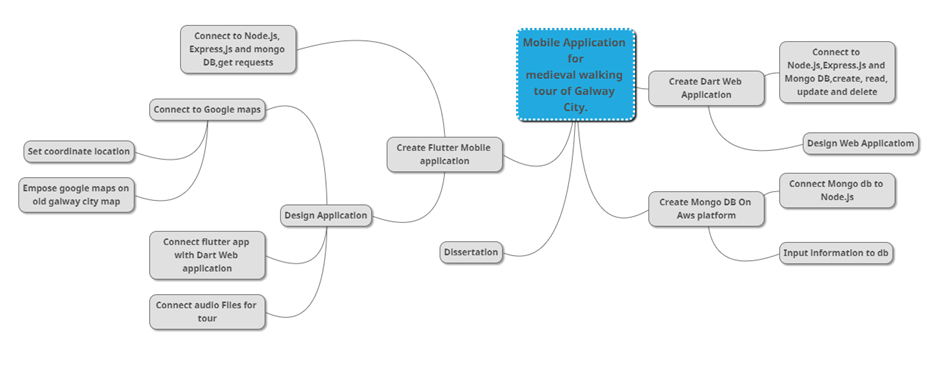
\includegraphics[width=135mm, height=50mm,scale=0.5]{img/plan.png}
\caption{Project Plan}
\label{fig:Project Plan}
\end{figure}

\subsection{Managing Project}
In order to manage this project GitHub was used. This was very useful due to it being a team project. It enables both members of the team to work on separate individual branches. After each iteration, these branches were merged into the master branch. After each integration, the project was at a working state of the project. This could be used for industry standard as continuous delivery. For this project it meant that after each sprint there was a working version to present to customer and supervisor. Although it is a working version is may still need changes in the next sprint. At the beginning of each sprint all branches pull from the master so as every team member is working off the same latest release of code.
\section{System Architecture}
\section{Technologies}
\subsection{Server}
\subsection{Client}

\subsubsection{Mobile Application}
Flutter was used to develop the cross platform mobile application for ios and android devices.Alot of research had to be carried out in order to learn dart programming language and learn the syntax of flutter along with understanding how widgets work correctly.When creating the the applications initially all pages were in one got class. This made the code very long and caused a lot of confusion.At this stage the developers decided to break up the code into a class for each location on the walking tour.

The main page holds the home page of the application along with the splashscreen of the application. The spashscreen widget has an initstate() method. This method calls the timer function which is an async method.The [callback] function is invoked after the given duration passed into the method. In order to display the images on the home page. A widget.dart page was created to hold stateless widgets foe each of the images on the main page. These widgets are then called by the main page. The main page imports each of the alternate pages at the top of the class. eg."import 'package:testing/walls.dart';".

The maps page contains all elements for the google maps used within the application.The map view library is imported at the beginning of the file.This enables the creating of a googles maps image in the application. This google maps image however is places on top of the widget. This was one of the largest problems experiences in the flutter development of the project. The map view is a separate widget that in linked to directly from google maps api. This is called from within a stateless widget. When the back button is selected the used is returned to a empty page. For used friendlyness a message to go back one more page is presented to the user.Flutter has a built in stateless widget called Marker. This enables a specific location to stand out on the map and when clicked a label appears over the marker.The Marker method takes the parameters (String id, String title, double longitude ,double latitude).The maps page is called by each of the location pages.

Each page containing the locations of the tour are layed out in similar format. Each file contains 2 stateful widgets. One of theses is the initial page for the location.This page contains multiple photos in a scrolling slide show. This user must select previous/next button to navigate though the images. The images are stored in a list and list is controlled by a photo Index to see what number of the list is currently being displayed.The text for each page is taken directly from the mongo flask database.The url location that the information from the database. The second stateful widget contains more detailed information about each location. This information was provided by Galway Civic trust and is based on the information in "Galway City medieval walk" booklet available at the hall of the red earl.The images included in this booklet are also in the application in similar format.

\subsubsection{Web Application}

\section{System Integration}
Due to this project being produced in conjunction with Galway Civic Trust, working closely with Michael Quinn to produce the exact item he wishes to publish is necessary. In order to do this Software Engineering techniques are being used to ensure the customer receives exactly what’s needed. The main approaches used are test driven development (TDD), behavior driven development (BDD) and user storyboards.

\subsection{Storyboards}

Storyboards were used to allow the customer give the developer’ss a high level view of expected design of the application. This is done using a blank page and the customer draws a simple representation of what they want the application to look like. This gives the developers a better understanding and idea what needs to be done and can help break down upcoming tasks to be completed. The storyboard used is taken from the agile methodology and is continuously being referred to and brought to each meeting with the customer to ensure every design requirement is clearly met. \cite{StoryBoard}

\subsection{Behaviour Driven Development}

Behaviour driven development is another agile software development methodology. It is designed based on what the user wants and how the user explains what the visual display of the application should look like. The customer/user gives a list of behaviours they wish the application be able to accomplish. These simple requests become a task or multiple tasks for the developer. When the application is complete the original requirements are made into unit tests.\cite{BDD} 

\subsection{Test Driven Development}

Test Driven Development is based predominantly on unit testing. However they are very different because test driven development is when the unit tests are written before the code has been created. This means the developers are using the unit tests as a guild and the tests alone break down the overall task needing to be completed. The tests will initially fail and the developers write minimal code in order for the tests to pass. This is process in continuously repeated in order for the application to pass each test. These tests are commonly automated.\cite{TDD}

\chapter{Results}
\section{Results of the Application}

\section{Testing}
Testing is an essential part of any software development life cycle. The importance of testing in software development life cycle is to improve reliability, performance and other important factors.\cite{TestingLifeCycle} Each component of the project can be tested individually.

\subsubsection{Test Plan}
A test plan consists of a list of scenarios and exact instruction of what needs to be tested in a project. The test plan must state exactly the features that need to be tested, the method in which they will be tested, the order these tests should be carried out and a time frame for these tests. The time frame ensures that testing is not left too late in the product life cycle.\cite{testPlan}
 
\subsubsection{Unit Tests}

Unit tests are individual tests to check functions, methods or classes. A test library is imported into the Flutter application. The developer/tester can run the unit tests from the terminal to check for success or failure. Unit tests can test that visual aspects of the application are working correctly along with connection to the backend database.

\subsubsection{Widget Testing}

A widget test exercises a single widget. Testing a widget involves multiple classes and requires a test environment that provides the appropriate widget life cycle context. \cite{testing}. It tests that the widget user interface performs as expected both visually and in it’s interactions. A widget should be able to check for user input and check for responses for the user based on actions performed. It is similar to unit testing because it tests the environment and is usually created to test certain actions alone.

\subsubsection{Integration Testing}

Integration testing is used to test the Flutter application as a whole. This tests that each function checked in unit and widget tests also work when incorporated with the remainder of the application. Integration testing is also used to test the performance of the application. This was done to test that the application could retrieve information from the database by many users simultaneously. Developers/testers can run the command "flutter driver" which sets up the test harness, builds and installs the application and runs the integration tests on the application. \cite{IntegrationTest}

\subsubsection{Fuzz Testing}
In order to carry out tests on the web application and mongo database, fuzz testing is used. This means testing the architecture by giving it a large variety of inputs. The web application updates, creates and deletes inputs from the Mongo DB. The input size is limited and this limit is tested to the max though fuzz tests, along with invalid inputs such as no input and numeric input alone. This testing is to be completed after the basic level of testing.

\begin{figure}[ht!]
    \centering
 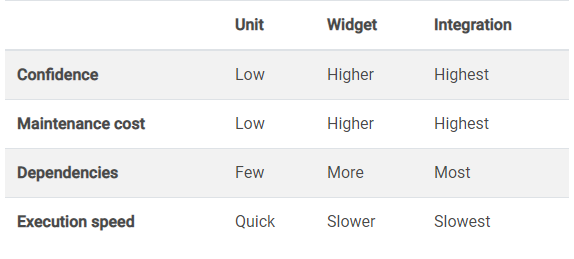
\includegraphics[width=125mm,scale=0.5]{img/Capture.PNG}
\caption{Testing:Types of testing}
\cite{testing}
\label{fig:method}
\end{figure}

\section{Complications}
\subsection{Flutter complications}
When creating the mobile application multiple problems were encountered. Many steps did not work as initially planned.
\subsubsection{Learning Flutter}
Learning flutter from basics was the first difficulty faced by the developers.However because flutter is built by google there are many open source online video and articles which help the learning process. Because of the developers knowledge of object oriented programming languages such as java it reduced the learning curve of flutter. However flutters widgets took longer than expected to fully understand and know when/how to use.

When Beginning the learning process of flutter the first place the developers looked was the flutter docs.\cite{flutterdocs} The official documentation flutter has provided for its developers is very good.It includes easy step by step examples of nearly every favourable scenario. The documentation is broken up into "flutter for android devs", "flutter for ios devs" , flutter for react native devs", "flutter for web devs".This breakdown enables developers to relate to flutter from different perspectives based on previous knowledge.The developers also came across a Youtube channel called MTechViral.\cite{channel_youtube} This channel posts videos on mobile development and have a flutter playlist. This YouTube channel is very popular and therefore a great place to communicate to other developers and learn from their experiences also.

\subsubsection{Incorporating google maps}
There was a lot of research put into incorporating google maps into the application correctly.When the developers began this process there was limited documentation on google maps integration to flutter applications.

In order to incorporate google maps into the application, there are multiple steps that must be followed.In order to use google maps within a flutter application,the \texttt{google\_maps\_flutter} plugin must be added as a dependency in the pubspec.yaml file of the application.Each developer must get a unique api key from google cloud platform.\cite{googleCloudMap}.The api key must be identified in the android application manifest and the ios application delegate. The google maps plugin allows the googlemap widget be added to a widget tree and map view is controlled by the google maps controller. This however has limitations, there are no markers supported.

The map attempted is \texttt{map\_view} plugin however this was not ideal due to the fact that is open the map within the application page but instead create a page ontop of the page and in order to go back to the previous page the user must press the back button on an adroid device or manually shut the application on an ios device. This was not very user friendly.A toolbarAction page has been added to ensure the ability to go back to the previous page.This is not working currently.

\subsubsection{Navigation between pages}
Flutter is unique with its use of widgets. In order to navigate between pages of a flutter application there must exist two or more routes. To switch to a new route the navigator.push() method must be called. This allows the new route to be added to the stack of routes managed by the navigator. In order to return to the previous route of an application the navigator.pop() method is called. This method removes the current route from the stack. In order to access a route that is in a different .dart file the correct file containing the route must be importing at the top of the .dart page.


\chapter{Conclusion}

 






 


